\section{Methods}
\label{sec: method}

\subsection{Global Attention Framework}
In an RNN encoder-decoder framework without attention mechanism, the RNN encoder reads the input sentence word by word and recursively updates its hidden state according to the previously hidden state and the current token's embedding.
As a result, the final hidden state vector is used as a summarized representation of the input sentence.
The decoder then takes the final hidden state vector as input and recursively chooses the token with highest probability from the vocabulary distribution until an end-of-sentence (EOS) token is obtained. This approach starts to deteriorate for longer input sentences because the summarization capacity of the encoder's final hidden vector is limited. 
Therefore, we adopted the global attentional encoder-decoder framework introduced by \cite{luong2015effective} because the news headline summarization task often has long input sentences. 

\begin{figure}
\centering
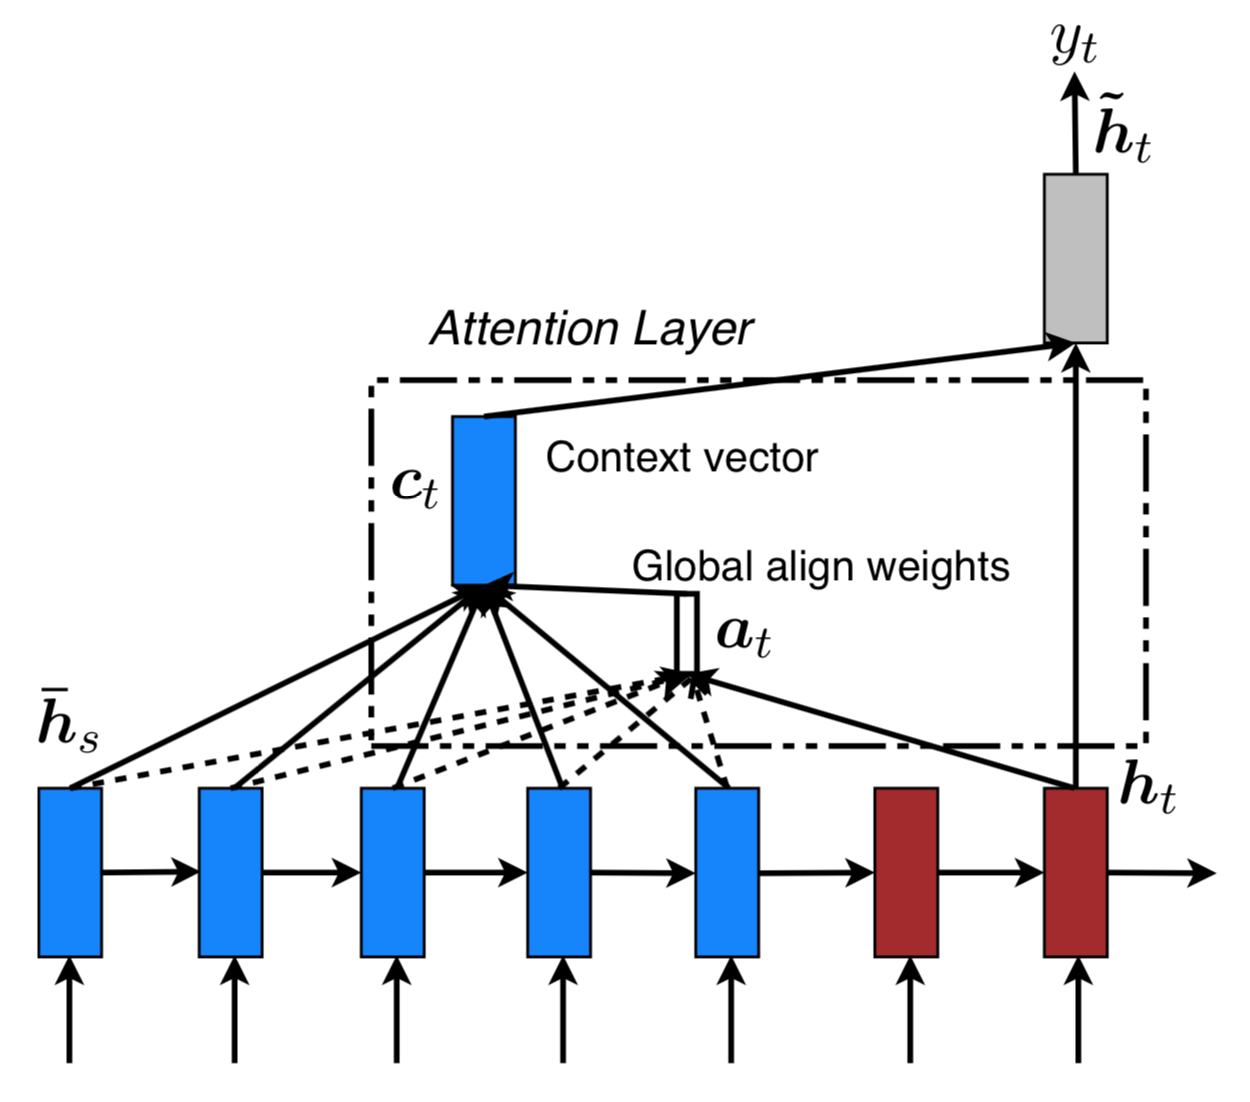
\includegraphics[width=\linewidth]{figures/luong2015.png}
\vspace{-8mm}
\caption{\textbf{Global attentional model}. The encoder computes an attention augmented hidden vector $\bm{\tilde h}_t$ by the context vector $\bm{c}_t$ and the current decoder vector $\bm{h}_t$. The context vector $\bm{c}_t$ is computed by
scoring each encoder hidden state vector $\bm{\bar h}_s$ by the current decoder hidden state $\bm{h}_t$ and taking a weighted average of the input hidden states using the attention weights $\bm{a}_t$ from the normalized scores. The figure is from the original paper \cite{luong2015effective}.}
\label{fig: luong2015}
\end{figure}

\small
\begin{align}
    score(\bm{h}_t, \bm{\bar h}_s) =
  \begin{cases}
        \bm{h}_t^T \bm{\bar h}_s & dot \\
        \bm{h}_t^T \bm{W_a} \bm{\bar h}_s & general \\
        \bm{v}_a^T tanh(\bm{W_a} [\bm{h}_t;\bm{\bar h}_s]) & concat 
  \end{cases}
  \label{eq: score}
\end{align}
\normalsize

In a nutshell, as shown in Fig. \ref{fig: luong2015}, \cite{luong2015effective} augmented the encoder RNN with a global attention mechanism to provide better summarization of the input sequence. Suppose that the decoder would like to sample a token at discrete time $t$. It first computes the current decoder hidden state $\bm{h}_t$ based on the previous decoder hidden state $\bm{h}_{t-1}$ and the previously chosen token. Then it scores each encoder hidden state $\bm{\bar h}_s$ for the input token $s$ using a score function. Some score functions are provided in Eq. \ref{eq: score}. In particular, we adopt the dot product score function for its computational efficiency. The attention weights over the input tokens are the softmax-normalized version of the scores. To decode each token from a decoder hidden state, this scoring procedure allows us to decide how much attention each input token needs. Using the encoder input token hidden states $\bm{\bar h}_s$ and the attention weights $\bm{a}_t$, the context vector $\bm{c}_t$ is obtained by a sum of $\bm{\bar h}_s$ weighted by $\bm{a}_t$. As a result, the context vector $\bm{c}_t$ has encoded attentional information of the input sentence. Finally, we concatenate the context vector $\bm{c}_t$ and the current decoder hidden state vector $\bm{h}_t$ and map to a vector $\bm{\tilde h}_t$ such that $\bm{\tilde h}_t, \bm{h}_t, \bm{c}_t$ share the same dimension.


\subsection{ELMo Embedding}
For model input, we use a pre-trained \texttt{ELMo} language model \cite{peters2018deep} to generate 256-dimension embeddings for our vocabulary. As discussed earlier, \texttt{ELMo}'s main advantage is its ability to generate contextualized word embeddings. In other words, it is able to generate a different embedding for the same word that appears in different contexts. This is crucial as it allows our text summarization model to disambiguate between multiple meanings of a given word, but the implication is that we can no longer use a fixed dictionary as a pre-trained embeddings input. To address this issue, we run every sentence in our training set through the pre-trained \texttt{ELMo} model, and save the average of all the embeddings we receive for a given word. One may argue that by taking the average -- thereby having the same embedding for a given word regardless of its context -- defeats the purpose of employing the contextualized representation. However, we believe that the average essentially incorporates all the meanings of a given word into the same embedding, and therefore should do no harm in the downstream task. In Table \ref{tab: compare_embed}, we compare the results of the same architecture using \texttt{GloVe} embeddings, \texttt{FastText} embeddings and averaged \texttt{ELMo} embeddings. 

\subsection{Adaptive Softmax}
One of the main challenges in this work is handling the size of the dataset. Even after downsampling to retain only $60\%$ of the training data and replacing low frequency words, our vocabulary is still too large to fit into the GPU memory. The bottleneck is that when the decoder predicts the next word, it relies on the last fully connected layer to map from hidden space to the output space in order to perform softmax, which is the same size as our vocabulary. The number of model parameters then scales linearly with the size of the vocabulary due to the fully connected layer. To circumvent this issue, we use adaptive softmax which is an efficient approximation to the regular softmax function \cite{grave2016efficient}. This strategy is the most effective when the output space is large and highly unbalanced, which is consistent with our vocabulary. Adaptive softmax works by partitioning the output space into clusters depending on the label frequencies, and thus approximating the regular softmax in a hierarchical fashion. Since the word frequencies roughly follows the Zipf's law \cite{wilson1949human} where a large proportion of the articles is covered by only a small number of words in our vocabulary, it would make sense to prioritize the prediction of higher frequency words than the less frequent ones. 


